%!TEX root = ../Thesis.tex

\chapter{Grundlagen}
\label{cha:grundlagen}

In diesem Kapitel werden die für das Verständnis und die Durchführung der Arbeit benötigten
Grundlagenthemen vorgestellt. Nach einer kurzen Erläuterung der Möglichkeiten der Verkehrsanalysen
mittels Luftaufnahmen, wird daher darauf eingegangen, auf welche Weise die in dieser Arbeit verwendeten
Fahrzeugtrajektorien ermittelt werden.
Anschließend werden Methoden vorgestellt, welche zur Bereinigung der gewonnenen Daten verwendet werden können.
Als wichtiges Mittel zur Identifizierung von Fahrspuren aus Trajektorien werden zudem
verschiedene Cluster-Algorithmen und Distanzmaße vorgestellt.

\section{Verkehrsanalyse mittels Luftaufnahmen}
\label{sec:traffic_analysis}

% Beschreibung der Aus den Luftaufnahmen ermittelten (ermittelbaren) Werte
% Vorteile der Verwendung von Luftaufnahmen zur Erstellung von Verkehrssimulationen

\section{Rekonstruktion von Fahrzeugtrajektorien aus Luftaufnahmen}
\label{sec:position_extraction}

% Beschreibung des kompletten Vorgangs bis Bewegungsbahnen der Autos vorliegen
% Tracking --> World-Matching --> Glättung

Die in dieser Arbeit verwendeten Fahrzeugtrajektorien stammen aus der Anwendung ``Tracker-Application''
des MEC-View Teilprojektes \textit{Luftbeobachtung}. Nachfolgend wird beschrieben, wie diese aus den Videoaufnahmen
rekonstruiert werden.

Die Verfolgung von bewegten Objekten beziehungsweise Fahrzeugen, wird in der ``Tracker-Application'' mittels
\textit{Supervised Tracking} umgesetzt. Bei diesem Verfahren wird ein initial manuell ausgewählter Bildbereich
automatisch mit Hilfe eines erlernten Klassifikators verfolgt. Der Klassifikator muss hierbei zwischen
Fahrzeugen und der Umgebung unterscheiden können.
Das grundlegende Vorgehen dieses Tracking-Ansatzes ist in Abbildung \ref{fig:grund_tracking}
dargestellt und kann wie folgt beschrieben werden:

\begin{itemize}
    \item[a)] Verfolgtes Objekt befindet sich zum Zeitpunkt $t$ an bekannter Position $p_1$
    \item[b)] Zum Zeitpunkt $t+1$: Anwendung des Klassifikators auf Positionen um $p_1$
    \item[c)] Erstellen einer \textit{Confidence Map}, welche die Wahrscheinlichkeit darstellt,
                das verfolgte Objekt gefunden zu haben
    \item[d)] Updaten des Trackers auf Position des Maxima der \textit{Confidence Map}
\end{itemize}

\begin{figure}[H]
    \centering
    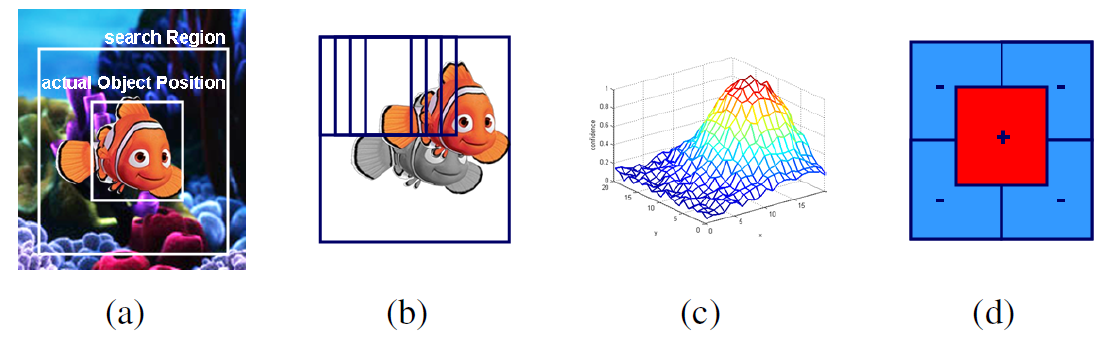
\includegraphics[width=0.7\linewidth]{../resources/img/grundlagen/tracking}
    \caption[Übersicht Tracking mit Klassifikator]{Übersicht Tracking mit Klassifikator \cite[]{Grabner}}
    \label{fig:grund_tracking}
\end{figure}

Das Erlernen eines stabilen Klassifikators in der ``Tracker-Application'' basiert auf der Arbeit
\textit{``Real-Time Tracking via On-line Boosting''} von \cite[]{Grabner}.
Die Autoren verwenden einen On-line AdaBoost Algorithmus, welcher mehrere \textit{schwache}
Klassifikatoren zu einem \textit{starken} Klassifikator kombiniert.
Schwache Klassifikatoren müssen hierbei nur eine Erkennungsrate von mehr als 50\% besitzen und somit
wenig besser als zufallsbedingtes Auswählen sein.
Starke Klassifikatoren entstehen durch die Kombination von mehreren schwachen Klassifikatoren.
Die Auswahl von schwachen Klassifikatoren erfolgt über sogenante Selektoren, welche aus einer Menge
immer jenen wählen, welcher die geringste Fehlerrate bei der Erkennung
der Trainings-Objekte besitzen. Der Klassifikator mit der schlechtesten Erkennungsrate wird in jeder
Trainingsiteration ersetzt, um das Training zu verbessern.
Großer Vorteil der On-line AdaBoost Methode ist, dass sie es ermöglicht, starke Klassifikatoren während des
eigentlichen Trackingvorganges zu erlernen. Nach jedem Trackingschritt wird das erfolgreich erkannte
Objekt in Trainingssätze zerlegt, auf welche die Klassifikatoren angewandt werden um ihre Performance zu evaluieren.
So wird in jedem Schritt die Menge der schwachen Klassifikatoren und der Selektoren aktualisiert. Die Wahl
von effizient berechenbaren schwachen Klassifikatoren macht dies möglich.

Die in \cite[]{Grabner} und der ``Tracker-Application'' verwendeten Klassifikatoren sind binär, das heißt,
sie teilen Objekte in die zwei Klassen \textit{erkannt} und \textit{nicht erkannt} auf.
Konkret werden Haar-ähnliche Bildmerkmale nach \cite[]{Viola} als schwache Klassifikatoren verwendet.
Diese sind ein Mittel zur Identifikation von Kontrastunterschieden in Bildern, welche sich sehr gut
zur Erkennung von Kanten und Linien eigenen. Ein Beispiel der Haar-ähnlichen Merkmale und ihres Einsatzes
bei der Gesichtserkennung ist in Abbildung \ref{fig:grund_hair_like} dargestellt.

Diese Merkmale werden als schwache Klassifikatoren mit zufälliger Skalierung, Größe und Position
auf dem Bild platziert. Sie suchen in dieser Region anschließend nach den von dem Muster definierten
Konturunterschieden. Eine Bereich gilt als erkannt, wenn der Betrag der Differenz der Pixelsumme des weißen und
schwarzen Bereiches des Musters unter einem festgelegten Grenzwert liegt.

\begin{figure}[H]
    \centering
    \subfloat[]{{
        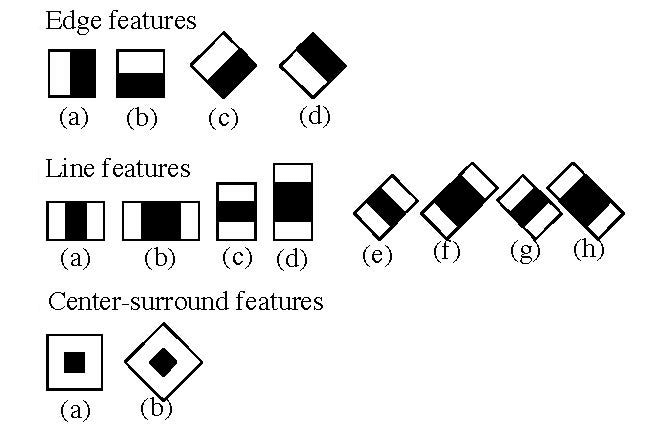
\includegraphics[width=0.4\linewidth]{../resources/img/grundlagen/hair_like_features}
    }}
    \qquad
    \subfloat[]{{
        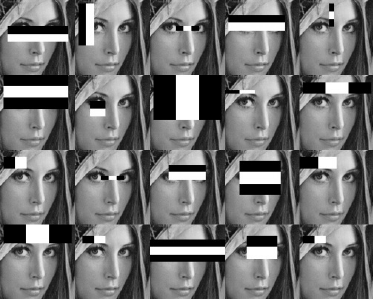
\includegraphics[width=0.35\linewidth]{../resources/img/grundlagen/hair_like_features_2}
    }}
    \caption[a) Haar-ähnliche Merkmale b) Beispiele für erkannte Regionen in einem Gesicht]{a) Haar-ähnliche Merkmale b) Beispiele für erkannte Regionen in einem Gesicht \cite[]{DivyanshDwivedi2018}}
    \label{fig:grund_hair_like}
\end{figure}

\section{Datenaufbereitung und Bereinigung}
\label{sec:tra_preprocessing}

% ALLGEMEINE Beschreibung von möglichen Datenbereinigungsschritten
% Resampling (Distanz oder Geschwindigkeit)
% Padding etc. (Interpolation)
% Glättung (RANSAC, Wavelet)

\section{Clusteranalyse}
\label{sec:tra_clustering}

Die Clusteranalyse (kurz Clustering) ist ein wichtiges Werkzeug zur Auswertung von Daten unterschiedlichster
Art. Sie stellt dabei kein konkretes Vorgehen oder einen Algorithmus dar, sondern beschreibt ein
allgemeines Problem, welches auf unterschiedlichste Weise gelöst werden kann.
Grundsätzlich ist das Ziel der Clusteranalyse, Datenobjekte aufgrund ihrer Eigenschaften und Beziehungen
untereinander so zu gruppieren, dass sich die Objekte einer Gruppe möglichst stark ähneln und sich
von den Objekten anderer Gruppen möglichst stark unterscheiden. Je höher die \textit{Homogenität} in einem Cluster
und die \textit{Differenz} zwischen den Clustern, desto besser ist die gewählte Clustering Methode.
Der Einsatz von Clustering ist in vielen Anwendungsgebieten und in den unterschiedlichsten wissenschaftlichen
Disziplinen sehr beliebt, um ein Verständnis für Daten zu erhalten beziehungsweise diese anschließend weiter
verarbeiten zu können.
So kommt die Clusteranalyse unter anderem in den Feldern des maschinellen Lernens, der Mustererkennung, Bildanalyse,
der Biologie (Taxonomie) oder im Bereich Data Mining zum Einsatz. \cite[]{tan2007introduction}

Die Clusteranalyse hat viel mit dem Problem der Klassifizierung von Daten gemein, insofern sie Datenobjekten
Label zuordnet. Im Gegensatz zu \textit{überwachten} Klassifizierungsansätzen, wie dem heute populären überwachten
Lernen, leiten Cluster-Algorithmen die Label allerdings alleine aus den vorhandenen Daten ab.
Es kommen keine Vergleichsobjekte mit bekannten, händisch vergebenen Labeln zum Einsatz.
Aus diesem Grund wird die Clusteranalyse auch häufig als \textit{unüberwachte Klassifizierung} bezeichnet. \cite[]{tan2007introduction}

Das Konzept eines \textit{Clusters} ist nicht genau definiert, was in einer Vielzahl an unterschiedlichen Ansichten
und Algorithmen resultiert, welche sich jeweils für andere Anwendungsfälle eignen und verschiedene Eigenschaften
besitzen. Hieraus ergibt sich auch die Tatsache, dass Clustering keine selbsttätiger Prozess ist, welcher sich auf
einheitliche Weise auf unterschiedliche Probleme anwenden lässt. Jedes Problem erfordert die individuelle und sorgfältige
Auswahl eines passenden Algorithmus, eines Distanzmaßes und der richtigen Parameter. Die Bestimmung dieser geschieht
iterativ und nicht selten nach dem Prinzip des \textit{Trial and Error}. In Abbildung \ref{fig:grund_clustering_example}
ist beispielhaft ein Datensatz (links) mit -- für den Menschen intuitiv ersichtlich -- 7 unterschiedlichen Clustern (rechts)
dargestellt. Nach \cite[]{Jain2010} kann allerdings kein verfügbarer Clustering Algorithmus diese alle erkennen.
\cite[]{Jain1999, tan2007introduction}

\begin{figure}[H]
    \centering
    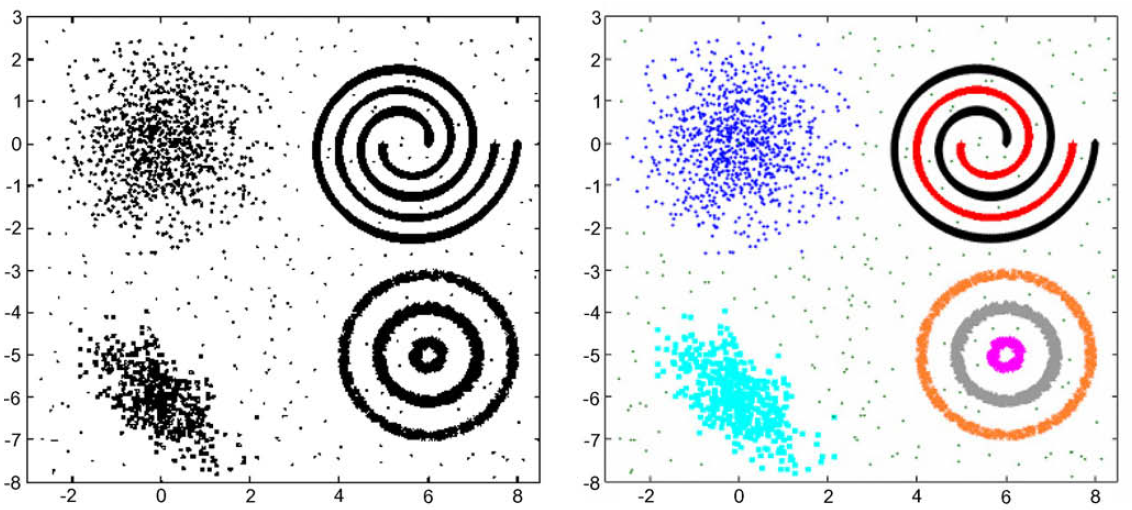
\includegraphics[width=0.8\linewidth]{../resources/img/grundlagen/clustering_example}
    \caption[Rohdaten (links) und erwünschtes Clustering-Ergebnis (rechts)]{Rohdaten (links) und erwünschtes Clustering-Ergebnis (rechts) \cite[]{Jain2010}}
    \label{fig:grund_clustering_example}
\end{figure}

Aufgrund der Limitationen, welche alle Cluster-Algorithmen besitzen, muss der Analyst sich vor deren Anwendung intensiv
mit den zu verarbeitenden Daten beschäftigen. Er muss ein Verständnis dafür besitzen, welche Struktur die Daten
besitzen, beziehungsweise annehmen können, und nach welchen Mustern zu suchen ist.
Besonders wichtiger ist zudem auch die Auswahl der richtigen, das heißt relevanten, Datenmerkmale (\textit{``Feature Selektion''})
und die Wahl deren Repräsentation (\textit{``Feature Transformation''}).
Die Selektion und gegebenenfalls Transformation der Daten muss in einem
Vorverarbeitungsschritt geschehen, dessen Qualität einen maßgeblichen Einfluss auf das finale Clustering Ergebnis hat.
Basierend auf vorangegangener Beschreibung und \cite[]{Jain1999}, lässt sich der Ablauf einer Clusteranalyse wie folgt darstellen:

% TODO: Grafik selbst neu erstellen
% (Feature Selection --> Feature Transformation --> Ähnlichkeitsmessung --> Clustering --> Feedback)
\begin{figure}[H]
    \centering
    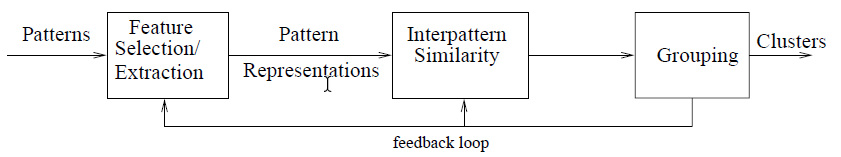
\includegraphics[width=0.8\linewidth]{../resources/img/grundlagen/clustering_workflow}
    \caption{Ablauf einer Clusteranalyse}
    \label{fig:grund_clustering_workflow}
\end{figure}

\cite[]{Jain2010} nennt einige weitere Herausforderungen, welchen man sich bei der Clusteranalyse bewusst sein muss:

\begin{itemize}
    \item Daten können Ausreißer enthalten. Wie sollen diese behandelt werden?
    \item Die Anzahl der Zielcluster ist üblicherweise nicht bekannt.
    \item Validierung der gefundenen Cluster
\end{itemize}

\subsection{Eigenschaften von Cluster-Sets und Clustern}

Das aus einer Analyse resultierende Cluster-Set und die einzelnen Cluster selbst,
können in verschiedene Kategorien unterteilt werden beziehungsweise unterschiedliche Eigenschaften besitzen.
Nachfolgend sind die wichtigsten basierend auf \cite[]{tan2007introduction} und \cite[]{Jain1999,Jain2010} aufgeführt.

\subsubsection{Cluster-Sets}

Bei Cluster-Sets kann grundsätzlich zwischen nachfolgenden Eigenschaften unterschieden werden.

\paragraph{Hierarchisch vs. Partitioniert}
Von \textit{hierarchischen} Cluster-Sets wird gesprochen, wenn die einzelnen Cluster verschachtelt sind und dabei eine
Baum-Struktur bilden. Cluster sind hingegen \textit{partitioniert}, wenn keine Überlagerungen zwischen ihnen existiert.

\paragraph{Exklusiv vs. Überlappend vs. Fuzzy}
\textit{Exklusive} Cluster-Sets liegen vor, wenn jedem Datenwert ein oder kein Zielcluster zugeordnet wird.
Im Gegensatz hierzu können bei \textit{überlappenden} Cluster-Sets Objekte einer oder mehrerer Gruppen angehören.
Bei dem sogenannten \textit{Fuzzy} oder \textit{Soft} Cluster-Sets, gehört ein Datenobjekt einem Cluster
mit einer bestimmten Wahrscheinlichkeit oder Gewicht an. Algorithmen, welche Daten eine
Wahrscheinlichkeit für die Zugehörigkeit zu einem Cluster zuweisen, werden \textit{probabilistische}
Cluster-Algorithmen genannt.

\paragraph{Komplett vs. Partielle}
Von \textit{kompletten} Cluster-Sets wird gesprochen, wenn jedes Element der Eingangsdaten einem Cluster zugeordnet wird.
Bei \textit{partiellen} Sets ist dies nicht der Fall. Hier kann ein bestimmter Anteil an Datenwerten als Ausreißer markiert
werden, welche keine Gruppe besitzen.

% TODO: evtl. Bild einfügen

\subsubsection{Cluster}

Da, wie oben erwähnt, nicht klar definiert ist, was ein Cluster ausmacht, können auch diese unterschiedliche Eigenschaften
besitzen. Die wichtigsten Cluster-Arten sind nachfolgend erläutert.

\paragraph{Klar separierte Cluster}
Unter \textit{klar separiereten} Clustern versteht man solche, in welchen jedes Datenelement einen geringeren
Abstand zu allen anderen Elementen des Clusters hat, als zu Elementen außerhalb des Clusters. Diese
idealistische Definition eines Clusters ist nur dann erfüllt, wenn die in den Daten enthaltenen Cluster einen
großen Abstand voneinander haben. Dies ist in der Realität allerdings selten der Fall.

\paragraph{Prototyp basierte Cluster}
Von einem \textit{Prototyp basierten} Cluster wird gesprochen, wenn alle Elemente einer Gruppe einen
geringeren Abstand zu einem Prototyp oder Referenzwert des Clusters besitzen, als zu denen anderer Gruppierungen.
Ein solcher Prototyp ist üblicherweise der Mittelwert der Datenelemente eines Clusters (\textit{Centroid}).

\paragraph{Graphen basierte Cluster}
Die Definition eines \textit{Graphen basierten} Clusters kann immer dann verwendet werden, wenn Daten
als vernetzter Graph dargestellt werden. In einem solchen sind die Elemente Knoten und die Kanten
repräsentieren Beziehungen zwischen ihnen. Ein Cluster in einem solchen Graphen ist definiert als Menge von
Knoten, welche untereinander verbunden sind, jedoch keine Verbindungen zu Elementen außerhalb des Clusters haben.

\paragraph{Dichte basierte Cluster}
\textit{Dichte basierte} Cluster sind definiert als Regionen mit einer hohen Dichte an Objekten, welche von
Regionen umgeben sind, welche eine geringe Objektdichte besitzen. Elemente, welche in einer solchen Region
mit geringen Dichte liegen, welche aus Ausreißer interpretiert. Dichte Bereiche werden üblicherweise
gefunden, indem die Nachbarschaften von Elementen untersucht werden.

\paragraph{Konzeptionelle Cluster}
% TODO: Verweis Bild hinzufügen
Eine sehr allgemeine Definition eines Clusters ist die der \textit{konzeptionellen} Gruppen. Hiermit ist
gemeint, dass die Elemente eines Clusters einige gemeinsame Eigenschaften besitzen. Dies schließt die oben genannten
Cluster-Arten mit ein, lässt sich allerdings beliebig erweitern. So sind beispielsweise in Abbildung XXX x)
konzeptionelle Cluster dargestellt, die die Form zweier Kreise und eines Dreiecks haben. Um solche Muster
erkennen zu können, würde ein Algorithmus eine besondere Definition eines Clusters benötigen.


% TODO: Bild hinzufügen und referenzieren

\subsection{Cluster-Algorithmen}
\label{sec:cluster_algos}

Um mit den oben beschriebenen unterschiedlichen Cluster-Set und Cluster Definitionen umgehen zu können,
existieren verschiedene Clustering-Modelle.
Einige wichtige Clustering-Ansätze sind die Vernetzungs-Modelle, Centroid-basierte-Modelle, Verteilungs-Modelle
oder Dichte-Modelle. Für jedes dieser Modelle existieren unterschiedliche Algorithmen. Im Folgenden werden
diese Modelle und jeweils exemplarisch ein Algorithmus der diese vertritt vorgestellt.

\subsubsection{Vernetzungs-Modelle}
% Agglomerative Hierarchical

Vernetzungs-Modelle werden auch häufig \textit{hierarchische Cluster-Modelle} genannt. Sie beruhen auf
der Annahme, dass Elemente, welche nahe beieinander liegen, eine höhere Gemeinsamkeit besitzen als solche,
welche weiter voneinander entfernt sind. Zur Bestimmung der Nähe zwischen Elementen benötigen Vernetzungs-Modelle,
wie auch andere Cluster-Modelle, eine
Definition von Distanz. Diese legt ein sogenanntes \textit{Distanzmaß} fest. Zusätzlich ist ein \textit{Link-Kriterium} notwendig,
welches bestimmt, wie genau die Entfernung zwischen zwei Clustern ermittelt wird. Übliche Link-Kriterien
sind \textit{Minimum-Linkage}, welches die minimale Distanz zwischen den Objekten der Cluster als Distanz verwendet,
oder \textit{Maximum-Linkage} beziehungsweise \textit{Average-Linkage}. \cite[]{Jain1999, GeorgeSeif2018}

Grundsätzlich teilen sich hierarchische Cluster-Algorithmen in zwei Gruppen auf:
\textit{Agglomerative} (Bottom-Up) und \textit{Divisive} (Top-Down) Algorithmen.
Agglomerative Ansätze weisen zu Beginn des Cluster-Vorgangs jedem Datenelement eine eigene Gruppe zu und vereinigen
diese anschließend.
Bei divisiven Ansätzen werden hingegen zu Beginn alle Elemente in einem Cluster zusammengefasst und
diese in den nachfolgenden Schritten geteilt.

Als Beispiel wird anschließend der \textbf{agglomerative-hierarchische Cluster-Algorithmus} genauer vorgestellt.
Sein Vorgehen lässt sich sehr gut anhand sogenannter Dendrogramme oder geschachtelter Cluster-Diagramme darstellen
(siehe Abbildung \ref{fig:grund_agglo_clustering})

% TODO: Bild selbst erstellen
\begin{figure}[H]
    \centering
    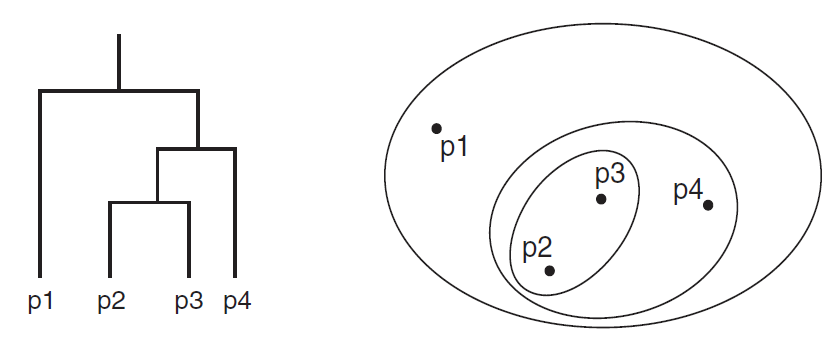
\includegraphics[width=0.7\linewidth]{../resources/img/grundlagen/agglo_clustering}
    \caption{Agglomeratives Clustering dargestellt als Dendrogramm und geschachteltes Cluster-Diagram}
    \label{fig:grund_agglo_clustering}
\end{figure}

Im ersten Schritt des Algorithmus werden alle Datenpunkte als separate Cluster markiert. Diesen Schritt
repräsentieren die Blätter des Dendrogramms.
Anschließend muss ein Distanzmaß und ein Link-Kriterium gewählt werden.
Das am häufigsten verwendete Distanzmaß ist sicherlich der euklidsche Abstand, welcher die Distanz zwischen zwei Punkten
oder Vektoren im $n$-dimensionalen Raum bestimmt. Er ist definiert durch die Formel \ref{eq_dist}.

\begin{equation}
\label{eq_dist}
    dist(p,q) = \|q-p\|_2 = \sqrt{\sum_{i=1}^n (q_i-p_i)^2}
\end{equation}

Wird als Link-Kriterium beispielsweise \textit{Minimum-Linkage} gewählt, ist dieses definiert als:

\begin{equation}
\label{eq_linkage}
    link(P, Q) = min\{ dist(p,q) : p \in P, q \in Q\}
\end{equation}

Hierbei entsprechen $P$ und $Q$ zwei Clustern, welche die Elemente $p \in P$ und $q \in Q$ enthalten.
Auf Basis des gewählten Link-Kriteriums kann nun eine Distanz-Matrix für die einzelnen Cluster
erstellt werden.
Die zwei Cluster mit minimalem Abstand voneinander werden anschließend zusammengeführt und die
vorherigen Schritte werden wiederholt, bis nur noch ein Cluster (Wurzel des Dendrogramms) beziehungsweise
die gewünschte Clusteranzahl übrig ist. \cite[]{GeorgeSeif2018, tan2007introduction}

Bei den meisten Varianten des agglomerativen Clusterings muss der Nutzer die Anzahl der Zielcluster im
vorraus festlegen, was problematisch ist, da diese meist nicht bekannt ist. Umgangen werden kann dies nur,
indem ein Link-Kriterium gewählt wird, das ab einer bestimmten Distanz zwischen den Clustern diese nichtmehr
fusioniert \cite[]{GeorgeSeif2018}.

Die Zeitkomplexität des agglomerativen Clusterings beträgt bestenfalls $O(m^2log\ m)$, weshalb die Menge der Daten,
welche mit ihm verarbeitet werden können erheblich begrenzt ist \cite[]{tan2007introduction}.

\subsubsection{Centroid-Modelle}

Centroid basierte Cluster-Modelle betrachten im Gegensatz zu hierarchischen Modellen nicht die Distanz
zwischen Clustern, sondern die Entfernung von Objekten zu Referenzpunkten, sogenannten \textit{Centroids}.

Ein Beispiel für einen Centroid-Cluster-Algorithmus ist \textbf{k-Means}. Dieser ist aufgrund seines Alters,
seiner Einfachheit und der vielen Weiterentwicklungen wohl der bekannteste Cluster-Algorithmus überhaupt.

Das Ziel von k-Mean ist es, für eine n-dimensionale Punktmenge $X = \{ x_1 ... x_n \}$ ein Cluster-Set $C = \{ c_1 ... c_k \}$
zu finden, welches die Summe der quadratischen Abweichung (Gleichung \ref{eq_kmeans1}) zwischen allein Punkten in einem Cluster und deren
Mittelwert $\mu_k$ (Centroids) minimiert.

\begin{equation}
    \label{eq_kmeans1}
    J(c_k) = \sum_{k=1}^K \sum_{x_i \in c_k} || x_i - \mu_k ||^2
\end{equation}

Eine Lösung für dieses Problem zu finden, ist NP-Schwer. Aus diesem Grund
ist k-Means ein approximativer Ansatz, welcher nicht garantieren kann, ein globales Minimum zu finden.
Die Funktionsweise des Algorithmus ist in Abbildung \ref{fig:grund_kmeans_clustering} dargestellt.
Die Kreuze entsprechen hierbei den Centroids.

\begin{figure}[H]
    \centering
    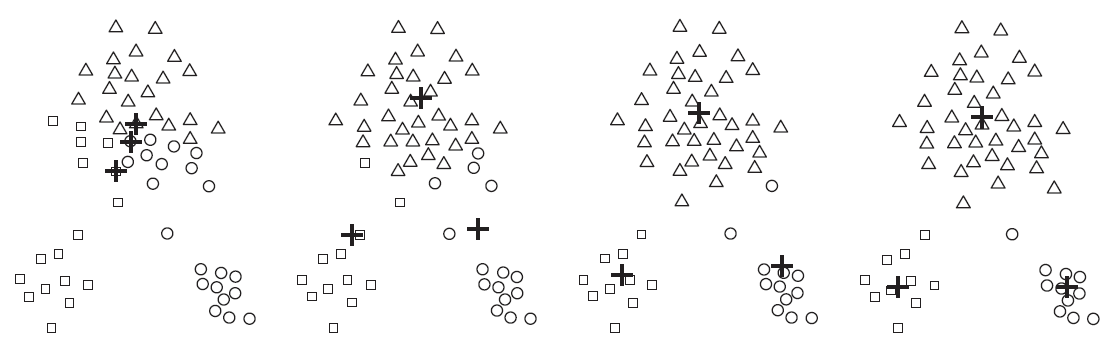
\includegraphics[width=0.9\linewidth]{../resources/img/grundlagen/k-means}
    \caption[Funktionsweise von k-Means]{Funktionsweise von k-Means \cite[]{tan2007introduction}}
    \label{fig:grund_kmeans_clustering}
\end{figure}

Ausgehend von der Punktmenge $X$ und der gesuchten Cluster-Anzahl $k$,
werden im ersten Schritt $k$ zufällig positionierte Centroids $\mu_k$ definiert.
Anschließend wird für alle Punkte $x_i$ der nächstgelegene Centroid $\mu_j$ gesucht.

\begin{equation}
    \label{eq_kmeans2}
    j = arg\ min(dist(x_i, \mu_j))
\end{equation}

$x_i$ wird daraufhin Mitglied in Cluster $C_j$. Als Distanzmaß ($dist$) kann hier wieder der euklidsche Abstand
(Gleichung \ref{eq_dist}) verwendet werden oder aber auch beliebige andere sinnvolle Metriken.
Nachdem alle Punkte $x_i$ einem Cluster zugewiesen wurden, werden die Centroid Positionen neu bestimmt.
Hierzu wird der Durchschnitt aller Punkte eines Clusters berechnet:

\begin{equation}
    \label{eq_kmeans3}
    c_j = \frac{1}{n} \sum_{x_j \in C_j} x_j
\end{equation}

Diese zwei Schritte werden mehrfach wiederholt, bis das Ergebnis konvergiert, das heißt die Zuweisungen sich
nurnoch geringfügig ändern. \cite[]{Jain2010}

Der primäre Nachteil des k-Means Algorithmus ist, das auch bei ihm die Anzahl der Zielcluster spezifiziert
werden muss. Desweiteren ist sein Ergebnis aufgrund der zufälligen Initialisierung der Centroids
nicht deterministisch. Vorteil von k-Means ist hingegen, dass seine Zeitkomplexität bei $O(n)$ liegt.

Um die genannten Nachteile, zumindest in Teilen, umgehen zu können, existieren diverse Weiterentwicklungen des k-Mean
Algorithmus. So stammen beispielsweise von \cite[]{Hamerly} und \cite[]{Pelleg} die Algorithmen \textit{g-Means}
beziehungsweise \textit{x-Means}, welche die Clusteranzahl $k$ auf Basis mehrerer k-Means Durchläufe und
statistischer Kennzahlen bestimmen.

\subsubsection{Distributions-Modelle}
% expectation maximization

Distributions-Cluster-Modelle basieren auf der Verwendung von statistischen Wahrscheinlichkeitsverteilungen wie
beispielsweise der Gauß-Verteilung. Cluster werden darüber definiert, wie wahrscheinlich es ist, dass Objekte
der selben Verteilung angehören. Problematisch ist die Verwendung dieser Cluster-Methodik, da sie anfällig für
das Problem des \textit{``Overfitting''} ist, wenn die Komplexität der verwendeten Modelle nicht beschränkt wird.
Zudem ist die Annahme, dass vielen realen Datensätzen ein statistisches Verteilungsmodell zugrundeliegt, gefährlich.
Ist diese These jedoch berechtigt, haben die Modelle den Vorteil, dass sie neben der Zuweisung von Objekten zu Clustern
auch Korrelationen zwischen einzelnen Attributen aufzeigen können. \cite[]{AndersDrachen2014}

Nachfolgend wird der bekannteste Vertreter der Distributions-Cluster-Algorithmen vorgestellt:
das \textit{Expectation–maximization} (EM) Verfahren unter Verwendung sogenannter \textit{Gaussian-Mixture-Models} (GMM).
Die Funktionsweise des EM-Algorithmus hat grundsätzlich viel gemein mit der des k-Mean Ansatzes.
Es wird ebenfalls mit einer festen Anzahl zufällig initialisierter Modelle gestartet, welche anschließend über mehrere Iterationen
an die Daten angepasst werden. Im Gegensatz zu k-Means, sind die gewählten Modelle hingegen Gauß-Verteilungen,
welche zwei Parameter besitzen: ihren Mittelwert und die Standardabweichung.
Das Vorgehen des EM-Algorithmus ist nachfolgend, basierend auf \cite[]{GeorgeSeif2018}, beschrieben und in
Abbildung \ref{fig:grund_em_clustering} grafisch dargestellt.

\begin{description}
    \item[1)] Wahl der Clusteranzahl $k$ und Initialisierung der Gauß-Modelle für die entsprechenden Cluster.
    \item[2)] Berechnung der Wahrscheinlichkeit, dass ein Datenpunkt zu einem Cluster gehört. Je näher
              ein Datenpunkt dem Zentrum einer Gauß-Verteilung ist, desto höher die Wahrscheinlichkeit für dessen Zugehörigkeit.
    \item[3)] Basierend auf den Wahrscheinlichkeiten werden die Parameter der Verteilungen neu berechnet.
              Hierzu wird die gewichtete Summe der Datenpunkt-Positionen errechnet. Die Gewichte entsprechen dabei
              den Wahrscheinlichkeiten, dass ein Element zu einem Cluster gehört. Hierdurch werden die Gauß-Modelle automatisch
              den in den Daten enthaltenen Clustern angepasst.
    \item[4)] Wiederholdung der Schritte 2) und 3), bis das Clustering-Ergebnis konvergiert.
\end{description}

\begin{figure}[H]
    \centering
    \subfloat[Iteration 1]{{
        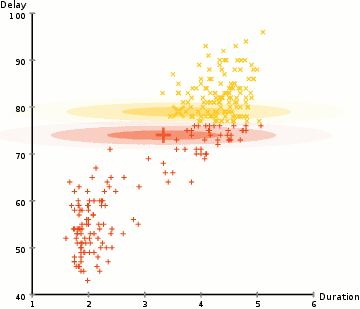
\includegraphics[width=0.22\linewidth]{../resources/img/grundlagen/clustering_EM/EM1}
    }}
    \subfloat[Iteration 2]{{
        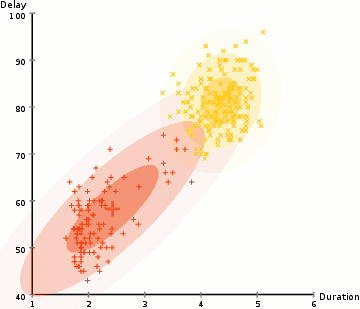
\includegraphics[width=0.22\linewidth]{../resources/img/grundlagen/clustering_EM/EM2}
    }}
    \subfloat[Iteration 3]{{
        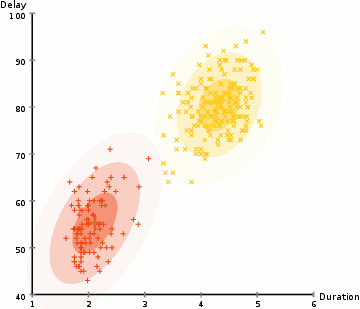
\includegraphics[width=0.22\linewidth]{../resources/img/grundlagen/clustering_EM/EM3}
    }}
    \subfloat[Iteration 4]{{
        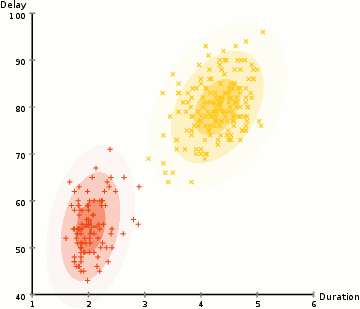
\includegraphics[width=0.22\linewidth]{../resources/img/grundlagen/clustering_EM/EM4}
    }}
    \caption[Darstellung des EM-Cluster-Algorithmus über mehrere Iterationen]{Darstellung des EM-Cluster-Algorithmus über mehrere Iterationen \cite[]{GeorgeSeif2018}}
    \label{fig:grund_em_clustering}
\end{figure}

Ziel des EM-Algorithmus ist es, die Parameter der Gauß-Modelle so zu optimieren, dass diese die Verteilung der Daten bestmöglich beschreiben.
Am Ende des Clusterings besitzt jeder Datenwert die Zugehörigkeit-Wahrscheinlichkeiten für die einzelnen Cluster.
Ein Element wird jenem Cluster zugeordnet, für welches es die höchste Wahrscheinlichkeit besitzt.

\subsubsection{Dichte-Modelle}

Dichte basierte Cluster sind, wie oben beschrieben, definiert als Regionen hoher Objekt-Dichte, welche
von Bereichen geringer Dichte umgeben sind. Dichte-Clustering-Modelle suchen nach eben solchen Regionen.
Großer Vorteil der Algorithmen dieser Klasse ist, dass sie Cluster beliebiger Formen finden können,
nicht auf die Vorgabe einer Clusteranzahl angewiesen sind und mit Ausreißern umgehen können.

Als Vertreter der Dichte-basierten Ansätze wird nachfolgend der \textbf{DBSCAN} Algorithmus
(\textit{Density-Based Spatial Clustering of Applications with Noise}), wie in \cite[]{Gao2012} beschrieben, vorgestellt.
Er verwendet als Maß für die Dichte einer Region die sogenannte \textit{$\epsilon$ -Nachbarschaft} (\textit{Eps}).
Diese selektiert für ein Objekt $p$ alle Objekte, welche innerhalb des Radius $\epsilon$ um dieses liegen:

\begin{equation}
    \label{eq_dbscan_1}
    N_{\epsilon}(p) = \{ q | dist(p,q) \leq \epsilon \}
\end{equation}

Eine $\epsilon$ -Nachbarschaft besitzt eine hohe Dichte, wenn in ihr mindestens $MinPts$ Objekte liegen.

Basierend auf der Definition von \textit{Eps}, werden die in einem Datensatz vorhandenen Elemente in
drei Klassen unterteilt. Sie sind entweder \textit{Kern-}, \textit{Rand-} oder \textit{Ausreißer-} Objekte.
Ein Kernobjekt hat mindestens $MinPts$ andere Punkte in \textit{Eps}.  
Randobjekte besitzen weniger als $MinPts$ in \textit{Eps}, liegen aber in der Nachbarschaft eines Kernobjektes.
Ausreißerobjekte sind weder Kern- noch Randobjekte.

\begin{figure}[H]
    \centering
    \subfloat[]{{
        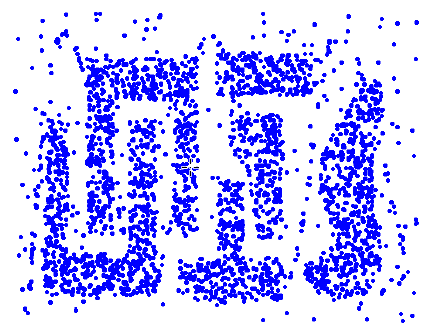
\includegraphics[width=0.3\linewidth]{../resources/img/grundlagen/clustering_dbscan/dbscan1}
    }}
    \subfloat[]{{
        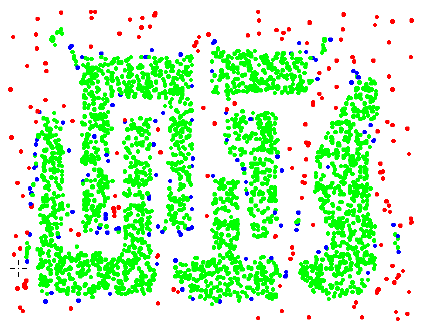
\includegraphics[width=0.3\linewidth]{../resources/img/grundlagen/clustering_dbscan/dbscan2}
    }}
    \subfloat[]{{
        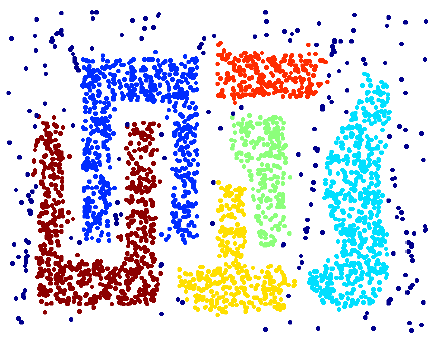
\includegraphics[width=0.3\linewidth]{../resources/img/grundlagen/clustering_dbscan/dbscan3}
    }}
    \caption[Schritte des DBSCAN Algorithmus]{Schritte des DBSCAN Algorithmus, a) Rohdaten, b) Klassifizierung in Kern- (grün), Rand- (blau) und Ausreißer- (rot) Punkte, c) Cluster Ergebnis \cite[]{Gao2012}}
    \label{fig:grund_dbscan_clustering}
\end{figure}

Auf Basis der drei Objektklassen, lässt sich das Prinzip der dichte-basierten \textit{Erreichbarkeit} definieren.
Ein Objekt $q$ ist von $p$ \textit{direkt} erreichbar, wenn $p$ ein Kernobjekt ist und $q$ in dessen \textit{Eps} liegt.
In Abbildung \ref{fig:grund_dbscan_reachability} gilt dies beispielsweise für $p$ und $p_2$.
Zwei Elemente sind \textit{indirekt} erreichbar, wenn sie über eine Reihe von Zwischenschritten (direkte Relationen)
verbunden sind (transitiv). Dies ist in Abbildung \ref{fig:grund_dbscan_reachability} für $q$ und $p$ der Fall.

\begin{figure}[H]
    \centering
    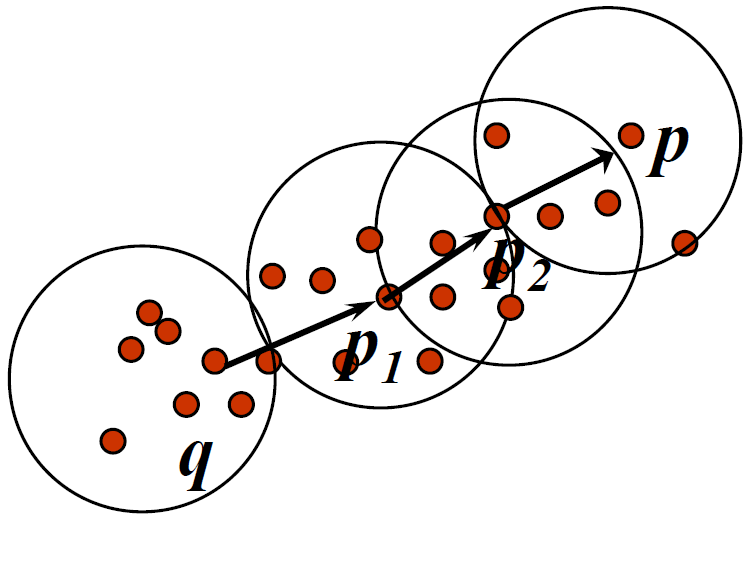
\includegraphics[width=0.32\linewidth]{../resources/img/grundlagen/clustering_dbscan/reachability}
    \caption[Erreichbarkeit in DBSCAN]{Erreichbarkeit in DBSCAN \cite[]{Gao2012}}
    \label{fig:grund_dbscan_reachability}
\end{figure}

Der DBSCAN Algorithmus lässt sich, basierend auf den obigen Definitionen, informell wie folgt beschreiben:

\begin{description}
    \item[1)] Unterteilung der Objekte in die drei Objektklassen. (Abb. \ref{fig:grund_dbscan_clustering} b))
    \item[2)] Aussortierung der Ausreißer-Objekte.
    \item[3)] Wahl eines nicht zugewiesenen Kernobjektes.
    \item[4)] Erstellung eines neuen Clusters für das Kernobjekt und alle von ihm ausgehend direkt oder indirekt erreichbaren Objekte
    \item[5)] Wiederholdung der Schritte 3) und 4), bis alle Kern- und Randobjekte einem Cluster zugewiesen sind. (Abb. \ref{fig:grund_dbscan_clustering} c))
\end{description}

DBSCAN besitzt die oben beschriebenen Vorteile Dichte-basierter Cluster-Algorithmen. Dank einer Zeitkomplexität
von $O(n log n)$ kann er außerdem auch auf große Datensätze angewendet werden.
Nachteil des Ansatzes ist hingegen, dass er schlecht mit Clustern umgehen kann, welche unterschiedliche Dichten besitzen. 

\subsection{Distanzmaße zum Vergleich von Fahrzeugtrajektorien}
\label{sec:distance_measures}

\section{Untersuchung möglicher Straßentopologien}
\label{sec:street_topologies}